\documentclass{standalone}
\usepackage{diplomski}

\begin{document}

\chapter{Data processing} \label{ch:data_processing}
\pagenumbering{arabic}
\setcounter{page}\thestranica

% --------------------------------------

\section{Data acquisition}

The data acquired by a DAQ card is processed in LabVIEW 2013 software by National Instruments. The same software solution is used to graphically display the results on the screen. DAQ cards produced by National Instruments are well supported in LabVIEW through an additional driver-toolbox. That, along with its advanced data processing capabilities, have places LabVIEW as a logical choice for this setup. \\

Data acquisition is performed in a while loop, during the entire program runtime. While repeating the loop, one must ensure that the DAQ card performs only data acquisition, and not system reconfiguration. Otherwise, acquisition time would greatly deteriorate. The \textit{NI-SCOPE} toolbox provides both an Express VI for data acquisition, as well as separate VI for a more hands-on configuration and acquisition approach. The implemented program uses an Express VI. The VI has an optional input \textit{Close}, which has to be connected to a False constant, to ensure the DAQ card is configured only on the first iteration of the while loop the VI resides in. \\

The data processing algorithm is displayed by a block diagram in Figure \ref{fig:program_block}.
\begin{figure}[h]
	\centering
	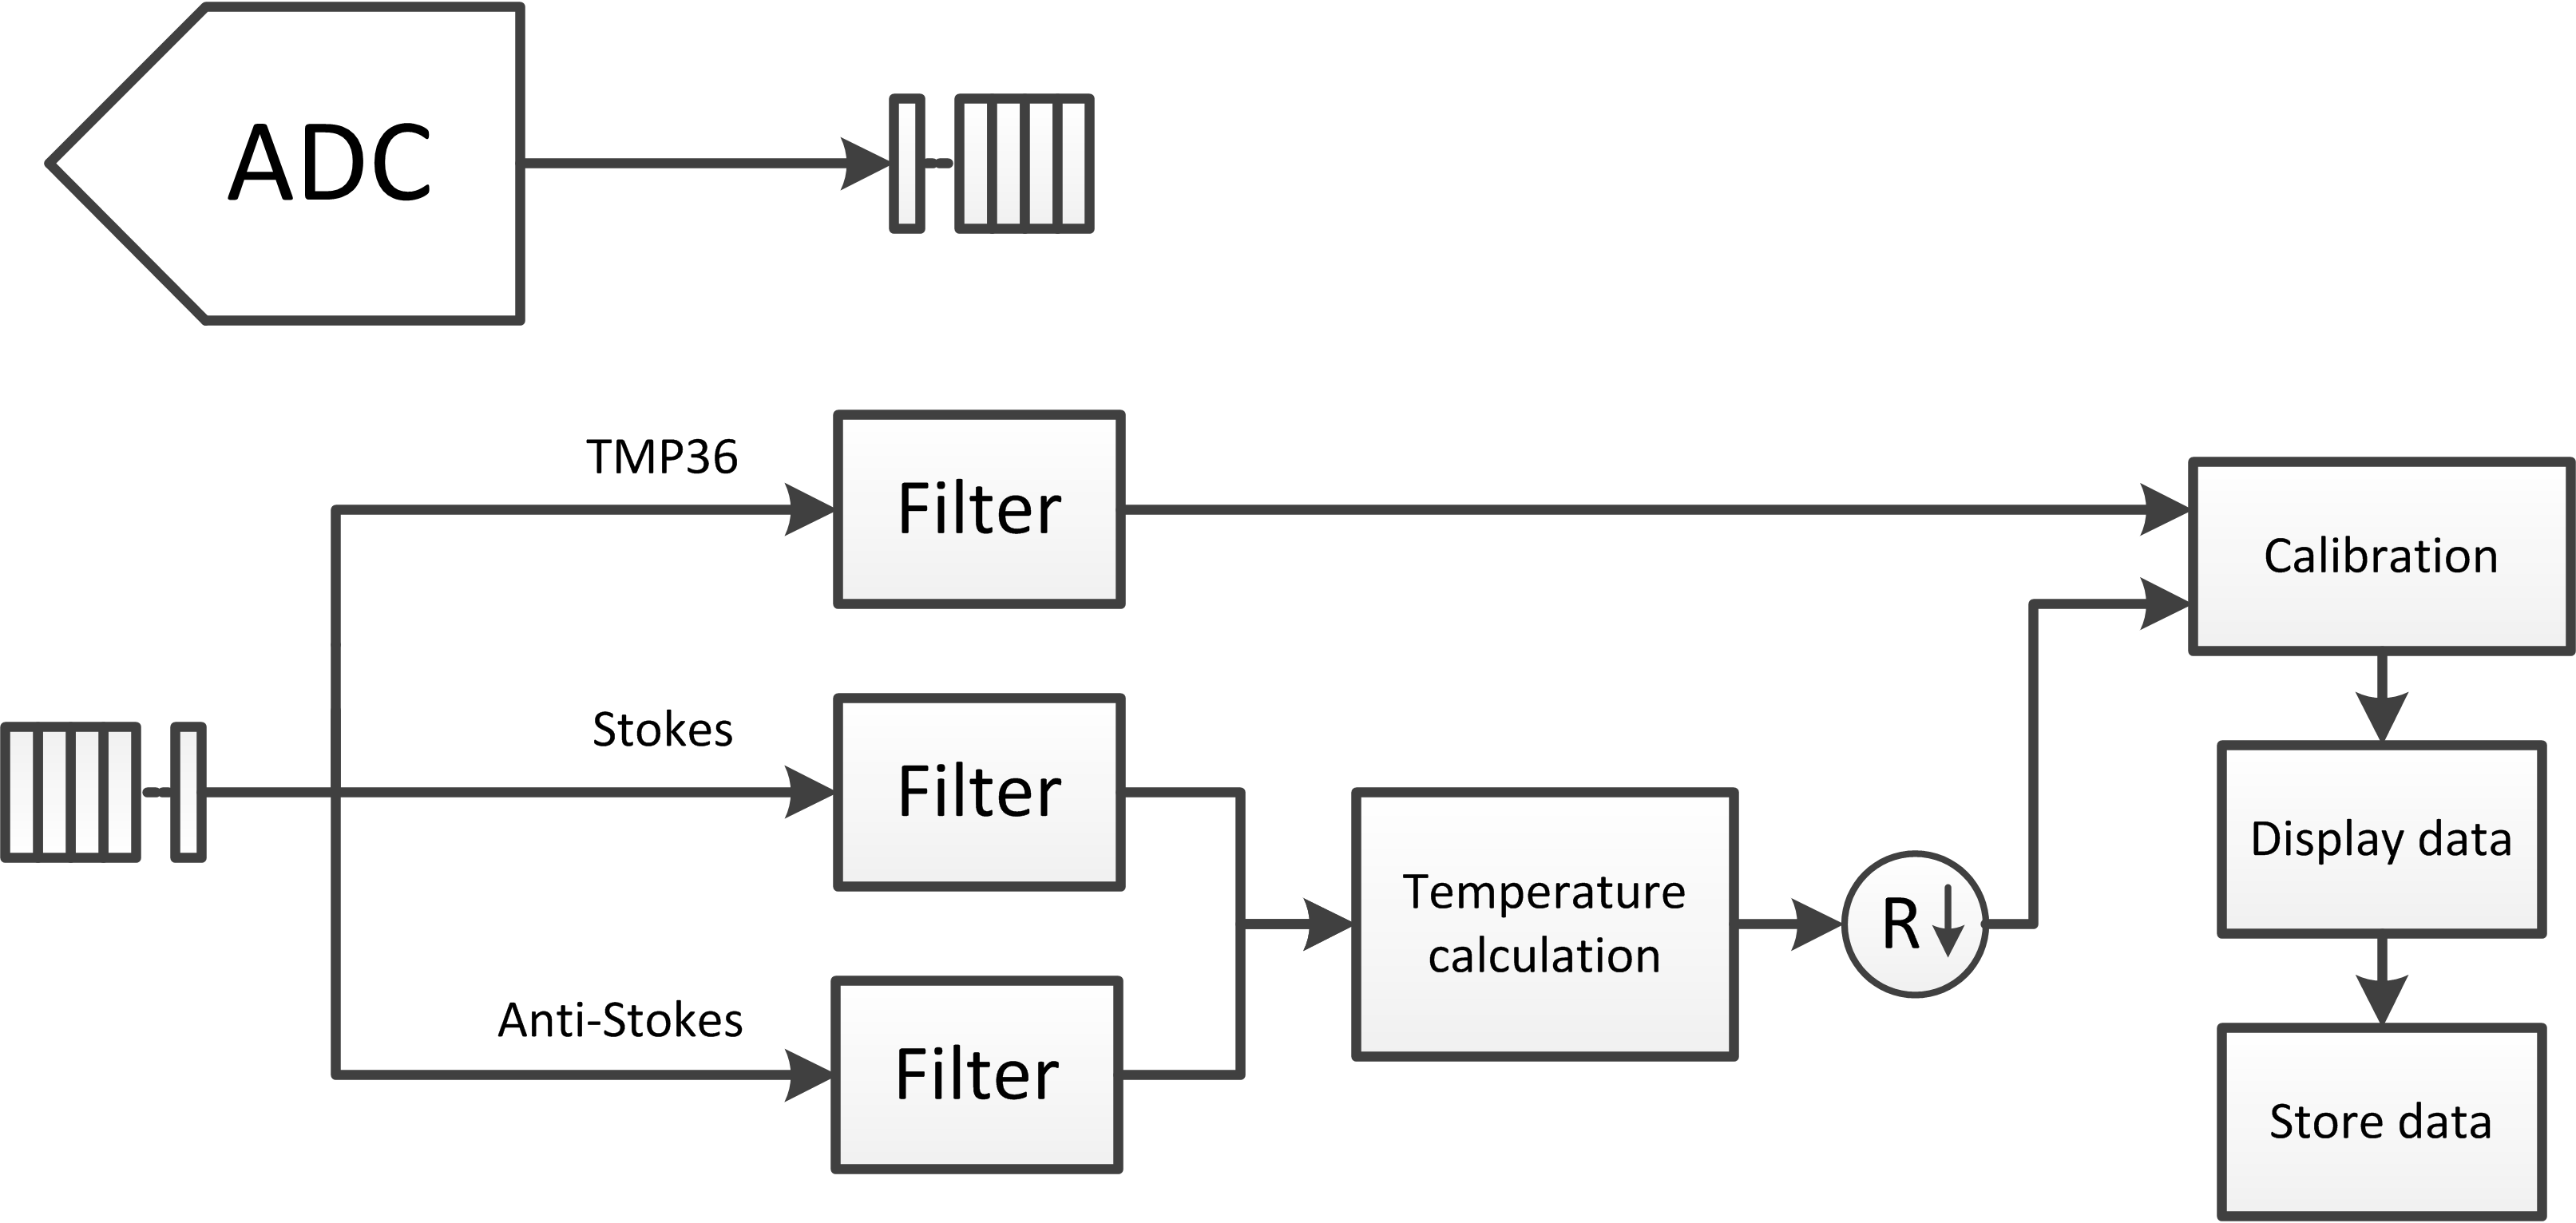
\includegraphics[width=\textwidth]{program_block}
	\caption{Block diagram of the data processing algorithm}
	\label{fig:program_block}
\end{figure}
In order to increase the processing speed, and so as not to skip any acquired samples, separate algorithms were developed, the one handling data acquisition, and the other for signal processing. The execution sequence is thus separated and handled by LabVIEW. Exchange of acquired data is performed by a queue structure. The queue is ensured to have a sufficient length to fit all the buffered data. LabVIEW inherently halts the data processing algorithm while the queue is empty, i.e. before the data is acquired from the DAQ device. \\

The DAQ card supports a maximum input signal frequency of 500 MHz \cite{datasheet:daq}, which corresponds to a minimum period
\begin{equation}
T_\textrm{min} = \SI{2}{\pico \second} \textrm{.}
\end{equation}
This ensures proper detection of source laser optical pulse, and is also well beyond the maximum bandwidth of used photodetectors. The acquisition memory length is set to 100000 samples. In this laboratory setup, this is enough to capture the signal backscattered from the end of the measurement fibre. It was observed that the DAQ card has a transient at the beginning of the acquisition windows. Therefore, the trigger, connected to the 1\% tap output of the laser, was set to be at the 50\% reference position, meaning that 50000 samples before the trigger, and 50000 samples after will be acquired. This is still enough to observe backscattering through the entire length of the measurement fibre. Channels connected to Stokes and anti-Stokes-monitoring photodetectors are AC-coupled to the DAQ card. This is to remove the DC bias of photodetectors that is of no interest in this system. Given the duty cycle of the optical pulse, the measured signal will still be around zero-value when it exits the range of the measurement fibre. However, additional zero-value correction is performed, which will be covered later on. \\

\section{Filtering}

As the monitored Stokes and anti-Stokes signals are very weak, they are highly noised at the photodetectors' output. By acquiring a large number of samples, and filtering the results, one can increase the SNR of measured signals. This will finally decrease the measured temperature error. While developing the data processing algorithm, several filtering algorithms were implemented and tested. Important characteristics of observed noise need to be taken into account while developing the algorithm. For the large part, the noise is white in character, and as such uncorrelated to the useful signal. \\

The first implemented algorithm is a simple averaging filter. The filter works well, and the measured temperature had a sufficiently low inaccuracy. However, the required averaging time to achieve this precision was more than 5 minutes. Therefore, this method was abandoned in favour of faster algorithms. The next implemented approach was an adaptive filter using the least-mean-square error (abbr. LMS) method. A block diagram of such a filter is presented in Figure \ref{fig:lms_block}.
\begin{figure}[h]
	\centering
	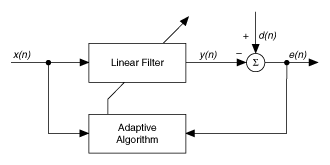
\includegraphics[width=0.7\textwidth]{lms_block.png}
	\caption{Block diagram of an adaptive filter \cite{labview:filter}}
	\label{fig:lms_block}
\end{figure}
The linear filter in the block diagram is an FIR filter. Its function can be expressed as \cite{anc}\cite{mitlecture25}
\begin{equation}
y(n) = x(n) \cdot w(n) \textrm{,}
\end{equation}
where $w(n)$ is the filter coefficient vector. The output signal $e(n)$ is the current error signal, and is in fact the difference between $y(n)$ and reference signal $d(n)$. Filter coefficients are updated by an adaptive algorithm. The algorithm compares the filtered signal with reference after each filter tap. Optimal coefficients are found so as to achieve the minimum mean square error with respect to the reference signal. Coefficients are calculated as
\begin{equation} \label{eq:normalizedlms}
w(n+1) = w(n) + \mu \, e(n) \, \frac{x(n)}{\| x(n) \| ^2} \textrm{.}
\end{equation}
Parameter $\mu$ is the filter parameter. Relation \ref{eq:normalizedlms} represents the normalized LMS algorithm. As the useful signal and noise are highly uncorrelated, an optimization by a large number of iterations would finally yield a filter that is a close estimate of the Wiener filter \cite{haykin2003least}. Ideally, the reference signal would be a response of the given measurement fibre under controlled conditions. Such a response could be obtained by a very large number of temperature measurements with a simple averaging filter. The measured data could be further de-noised by theoretically considering the characteristics of the specific fibre. This kind of calibration would require careful control of the measuring environment, and could prove to be a very time consuming process. Also, such a filter would result in a system calibrated only for a specific measurement fibre. Errors could occur just by reconnecting the system parts (e.g. reconnecting an optical connector of the measurement fibre). In many practical applications, it is proven sufficient just to use the delayed input signal as the reference. This approach requires multiple criteria on the observed signal to be met. Firstly, the signal should be stationary between a number of iterations. Furthermore, the signal and the noise we wish to filter out need to be uncorrelated. As the noise is dominated by white noise, this criteria is inherently met. Finally, in case the observed signal is narrowband, the noise is required to be broadband. Vice versa applies; If the signal is broadband, noise is required to be narrowband. The DAQ sampling rate is sufficiently large, and white noise is therefore spread across the entire discrete spectrum. Also, any kind of temperature shift will be mediated to the DAQ card by an optical pulse of short duration, its main spectral component residing at
\begin{equation}
f_0 = \SI{40}{\mega \hertz}
\end{equation}
for pulse duration
\begin{equation}
T_0 = \SI{25}{\nano \second} \textrm{.}
\end{equation}
We may assume any relevant temperature shift to be spectrally limited predominantly around $f_0$. Therefore, the former condition applies. This filter has proven its superiority towards a classic averaging filter. Some time is required for the adaptive filter to converge its coefficients and display the accurate absolute temperature value. However, overall averaging time required to obtain the same SNR is about one order of magnitude in seconds shorter than that of the classic averaging filter. \\

The approach applied for the two averaging algorithms is to use all the entire history of acquired samples while filtering. This requires low memory usage, as the once filtered samples may be removed from memory. However, such a system can not respond to a fast change in temperature, as averaging would filter the measured change out. To make a responsive system, one must first determine the averaging time, i.e. the number of averaged samples, required to obtain a desired SNR in measured signals. This will decide on the responsivity of the system. Next, a moving average filter should be implemented. Such a filter utilizes a \textit{filtering window}, taking only a predefined number of samples into account. This requires a large amount of memory, as all the samples in the filtering window need to persist for proper calculation. In an implemented prototype the processing time of each filter tap has proven to be extremely long, which is the result of a double float representation in LabVIEW of all the sampled data. This, along with the problem of high memory usage, has rendered this method impractical for use in current setup. \\

After filtering, waveforms are obtained, representing Stokes and anti-Stokes components in time. An example of acquired signals before and after filtering is given in Figure \ref{fig:daq_example}.
\begin{figure}[h]
	\centering
	\begin{subfigure}[b]{0.49\textwidth}
		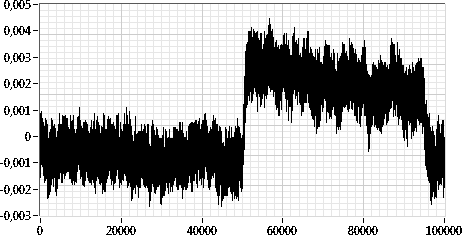
\includegraphics[width=\textwidth]{daq_example_stokes_current.png}
		\caption{Stokes channel, current value}
	\end{subfigure}
	\begin{subfigure}[b]{0.49\textwidth}
		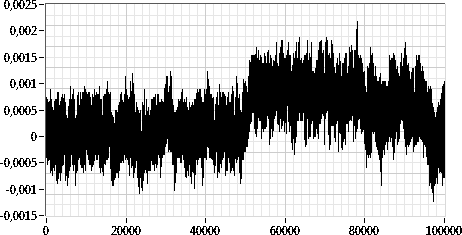
\includegraphics[width=\textwidth]{daq_example_antistokes_current.png}
		\caption{Anti-Stokes channel, current value}
	\end{subfigure}
	\begin{subfigure}[b]{0.49\textwidth}
		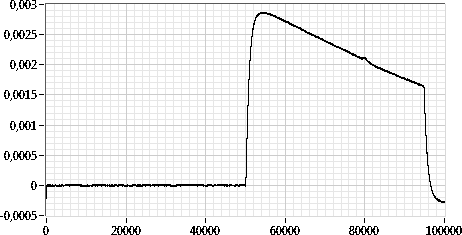
\includegraphics[width=\textwidth]{daq_example_stokes_filtered.png}
		\caption{Stokes channel, filtered value}
	\end{subfigure}
	\begin{subfigure}[b]{0.49\textwidth}
		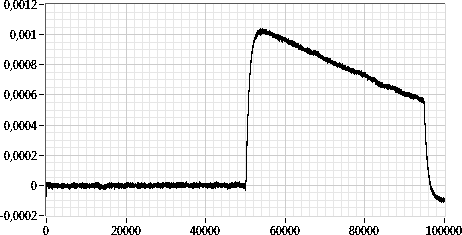
\includegraphics[width=\textwidth]{daq_example_antistokes_filtered.png}
		\caption{Anti-Stokes channel, filtered value}
	\end{subfigure}
	\caption{Filtering acquired signals}
	\label{fig:daq_example}
\end{figure}


\section{Temperature calculation}

The filtered Stokes and anti-Stokes profiles can be used to obtain the measurement fibre's temperature. A new LabVIEW virtual instrument was created for this purpose. It takes the measured signals as inputs, as well as some channel parameters, such as the effective scattering wavelengths that are entered manually, and ratios of gains between Stokes and anti-Stokes detection channels. The algorithm uses expression \ref{eq:stokes_temperature} to obtain the temperature. The energy shift is calculated from input parameters as
\begin{equation}
\varDelta E = \hbar (\omega_0 - \omega_\textrm{S}) \textrm{,}
\end{equation}
where $\omega_0$ is the optical frequency of the initial pulse, and $\omega_\textrm{S}$ the effective frequency of the Stokes component. The effective wavelength was input to the VI after theoretically calculating the effective wavelength of scattered signals. By using a high-sensitivity optical spectrum analyser, the effective frequency could be measured instead, to obtain a more precise value. The ratio of gains between Stokes and anti-Stokes detection channels is a sum ratio of all the different gain parameters found in measurement chains. Firstly, this includes photodetectors' responsivities, which are wavelength-dependent. Next, different photodetectors have different electrical gains, as presented in Table \ref{table:photodetectors}. All of these differences need to be either measured or taken from datasheets, and included in the ratio. \\

At different wavelengths, the measurement fibre will have different attenuation coefficients. If the attenuation coefficient difference is not compensated for, the temperature profile will have a slope, as the temperature and the scattering profiles are joined by a negative exponential function. In a controlled scenario, where the temperature along the measurement fibre is the same, one can apply classic OTDR methods to measure the fibre attenuation at different wavelengths. Figure \ref{fig:otdr_attenuation} is taken from a sample OTDR measurement. 
\begin{figure}[b]
	\centering
	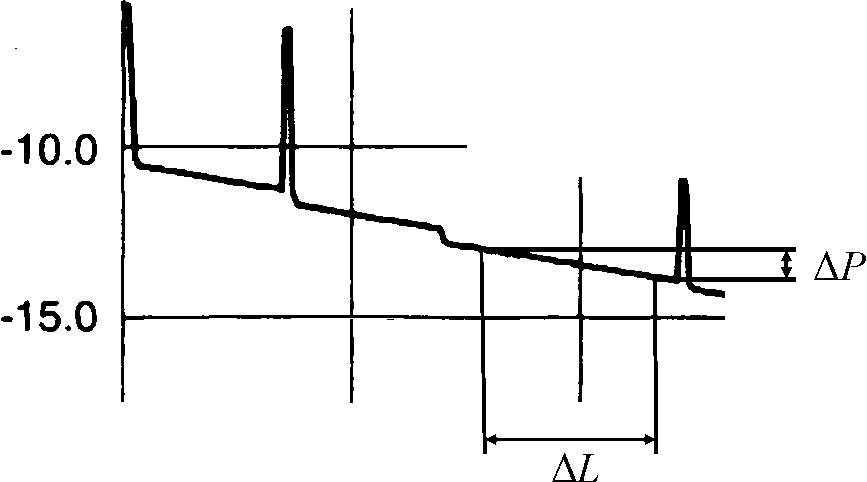
\includegraphics[width=0.7\textwidth]{otdr_attenuation.png}
	\caption{Measuring fibre attenuation coefficient \cite{fer:oks}}
	\label{fig:otdr_attenuation}
\end{figure}
The y-axis is in logarithmic scale. By measuring the slope of the curve, one can obtain the fibre attenuation at given wavelength as \cite{fer:oks}\cite{UnderstandingOTDRs2000}
\begin{equation}
\alpha \, \textrm{[dB/km]} = \dfrac{\varDelta P \, \textrm{[dB]}}{\varDelta L \, \textrm{[km]}} \textrm{.}
\end{equation}
The program takes attenuation coefficients at Stokes and anti-Stokes wavelengths, $\alpha_\textrm{S}$ and $\alpha_\textrm{AS}$, as input parameters. Assuming a linear change of attenuation coefficient with wavelength, one can now obtain $\alpha_0$ at laser wavelength and finally, the required attenuation difference due to frequency shift as
\begin{equation}
\varDelta \alpha_\textrm{P} = \alpha_0 - \alpha_\textrm{S}
\end{equation}
for Stokes channel and
\begin{equation}
\varDelta \alpha_\textrm{P} = \alpha_0 - \alpha_\textrm{AS}
\end{equation}
for anti-Stokes channel. \\

At this point, all the terms in \ref{eq:stokes_temperature} are ready and temperature profile can be obtained. An example profile is given in Figure \ref{fig:temperature_example}.
\begin{figure}[h]
	% Measurement 11.4.
	\centering
	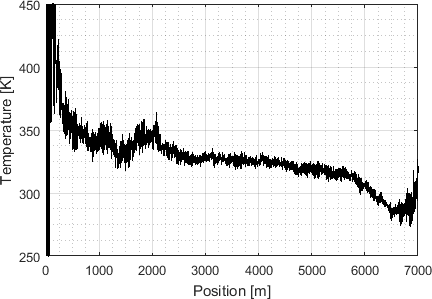
\includegraphics[width=0.8\textwidth]{temperature_example.png}
	\caption{Example temperature profile}
	\label{fig:temperature_example}
\end{figure}
One can observe a number of issues on the calculated profile, knowing that the measurement fibre was on room temperature. The measurement was conducted by using a cascade of a common G.652-compliant fibre, some 2.3 km in length, followed by a highly non-linear fibre, about 4.2 km in length. The x-axis represents the DAQ sample number. The y-axis is temperature in kelvins. It is clear that the fibre with expressed non-linearities provides a much more accurate temperature profile. Also, the measurement is offset from room temperature, as the correct terms from \ref{eq:stokes_temperature} are not known. An especially critical term is the effective wavelength of Stokes and anti-Stokes scatterings. At this point, reading from the discrete temperature sensor TMP36 is taken and samples at the beginning of the measurement profile are offset to match the measured temperature. However, one must take care not to calibrate on the part of the measured profile that represents the very beginning or the very end of the fibre. High reflections off optical connectors produce incorrect temperature measurement in these regions. Such errors could be mitigated by using better matching at the ends. Also, a trade-off can be found between the incident optical power and the resulting reflection. By calibrating against the discrete sensor, the calibration inaccuracy of the system will match that of the discrete temperature sensor. In this case, it is \cite{datasheet:tmp36}
\begin{equation}
\varDelta T = \SI{2}{\celsius}
\end{equation} \\

Additional correction can be performed in order to eliminate the apparent slope of the temperature profile. The slope is the result of an erroneous measurement of the attenuation coefficient difference. A slope in the resulting temperature profile can be measured, and rotated in post-processing. Next, the x-axis can be scaled using equation \ref{eq:otdr_time_distance} to represent length, rather than sample number. Another correction handles the incorrect data representation of the obtained temperature profile. The number of samples in the profile will be the same as the number of samples in the Stokes and anti-Stokes signal, as temperature is numerically calculated from them. Equation \ref{eq:otdr_resolution}, on the other hand, proves that the spatial measurement resolution is tied to the optical impulse width, rather than the sampling rate of the DAQ device. Decimation is performed on the acquired temperature profile to match the actual resolution of the measurement method. Decimation decreases the sampling rate of a discrete signal by removing extra samples from the signal. Averaging can be performed in the process, so that the data from extra samples is not lost. Decimation factor $R$ is taken as a ratio of original and target sampling rate, and in this case it can be expressed by the laser impulse width $T_0$ as
\begin{equation}
R = \frac{f_H}{f_L} = f_H \cdot T_0 \textrm{.}
\end{equation}
Given an example
\begin{equation}
f_H = \SI{1.25}{\giga S / \second}
\end{equation}
\begin{equation}
T_0 = \SI{25}{\nano \second} \textrm{,}
\end{equation}
the calculated decimation factor and the low sampling rate are
\begin{equation}
R = 31.25
\end{equation}
\begin{equation}
f_L = \SI{40}{\mega S / \second} \textrm{.}
\end{equation}
Sampling rates are given in samples per second for clarity. \\

Some of the suggested corrections were in fact removed from the final program version, as the processing time was too long. Different development platforms or system architectures could be used in future measurement systems, so as to implement better parallelism between the acquisition, basic processing and post-processing tasks of the measurement process.

\section{Data representation}

The user interface is presented by Figure \ref{fig:user_interface}. The interface features graphs representing the currently measured photodetector output signals, filtered Stokes and anti-Stokes components, source laser waveform and final temperature profile. Each graphs' x-axes represents the sample number, except for the temperature profile graph, whose x-axis is scaled to represent the location on the measurement fibre in metres. The y-axis on the temperature graph represents the temperature in kelvins, while other graphs' y-axes present the amplitude of the acquired analogue signal in volts. Numerical indicators at the bottom of the user interface display the calculated peak laser power in watts, peak amplitude at the output of the photodetector monitoring the 1\% tap output of the laser, as well as the reference temperature in kelvins, measured by the TMP36. To ensure accurate decimation of the temperature profile, user is required to input the laser pulse width, as configured in the laser's configuration interface. \\

Once run, the user interface redraws the acquired and calculated signals after every iteration of the data processing \textit{while} loop. The featured \textit{STOP} button will stop the program execution, while properly closing the DAQ device in the process. Furthermore, a user prompt dialogue will be displayed, allowing the user to input the filename for the comma separated value-formatted (abbr. CSV) output including filtered Stokes and anti-Stokes profiles, calculated temperature profile and last-acquired laser waveform. The CSV file enables further processing in other programming and data analysis environments.

\begin{landscape}
	\begin{figure}[h]
		\centering
		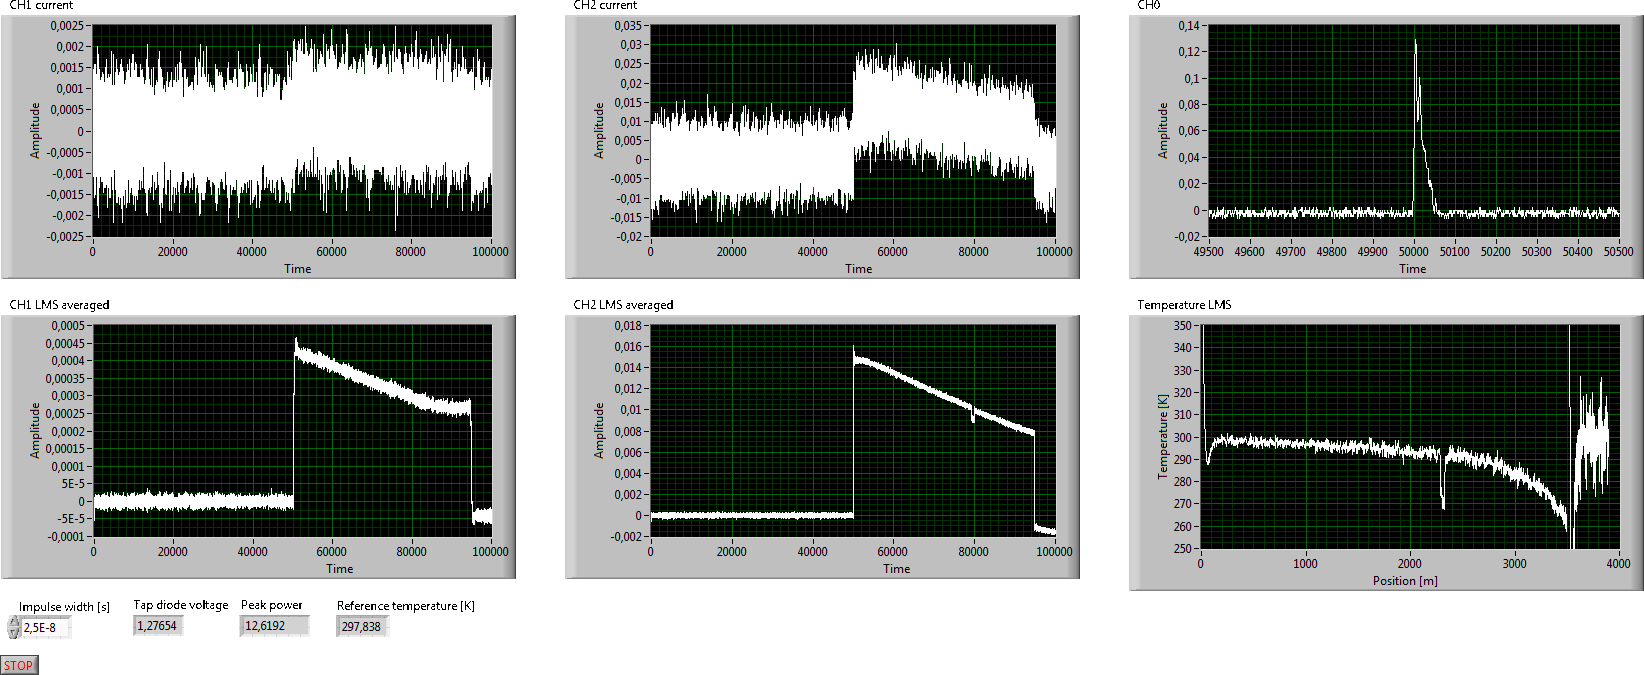
\includegraphics[width=1.05\linewidth]{user_interface.png}
		\caption{LabVIEW user interface}
		\label{fig:user_interface}
	\end{figure}
\end{landscape}

% --------------------------------------

\setcounter{stranica}{\thepage}
\addtocounter{stranica}{1}

\end{document}